\chapter*{Chapitre 2 : Cahier des Charges et Spécifications}
\addcontentsline{toc}{chapter}{Chapitre 2 : Cahier des Charges et Spécifications}
\thispagestyle{fancy}
\setcounter{section}{0}
\newpage

\section{Introduction}

Ce chapitre présente le cahier des charges et les spécifications du projet LearnExpert, une plateforme e-learning innovante développée au sein d'IAAI. Il détaille le contexte du projet, les objectifs visés, ainsi que l'analyse approfondie des besoins fonctionnels et non fonctionnels. Cette étape préliminaire est essentielle pour établir une vision claire du système à développer et pour guider efficacement les phases ultérieures de conception et d'implémentation.

Nous aborderons également les choix technologiques effectués pour répondre aux exigences du projet, en justifiant la sélection de chaque composant de la stack technique. Cette analyse des besoins et des technologies constitue le socle sur lequel reposera l'ensemble du développement de la plateforme LearnExpert.

\section{Présentation du Projet LearnExpert}

\subsection{Contexte et Problématique}
Le secteur de l'éducation en ligne connaît une croissance exponentielle, accélérée encore davantage par la pandémie mondiale qui a révélé les limites des plateformes d'apprentissage existantes. Dans ce contexte, plusieurs problématiques ont été identifiées :

\begin{itemize}
  \item Les plateformes actuelles proposent souvent un contenu générique et peu personnalisé
  \item Les méthodes d'apprentissage de la programmation restent trop théoriques, avec un manque d'interactivité
  \item Les apprenants font face à une fragmentation des ressources éducatives, nécessitant de naviguer entre différentes plateformes
  \item Les outils d'apprentissage ne s'adaptent pas au rythme et au niveau de chaque utilisateur
\end{itemize}

Face à ces défis, IAAI a décidé de développer LearnExpert, une plateforme innovante centrée sur l'apprentissage de la programmation et des technologies web.

\subsection{Objectifs du Projet}
Le projet LearnExpert vise à créer une plateforme d'apprentissage complète qui se distingue par :

\begin{itemize}
  \item Une approche centrée sur la pratique et l'interactivité pour l'apprentissage de la programmation
  \item Une personnalisation de l'expérience d'apprentissage grâce à l'IA
  \item Une intégration de contenus structurés et de haute qualité pour divers langages de programmation
  \item Une architecture évolutive permettant d'ajouter de nouvelles fonctionnalités et de nouveaux contenus
  \item Une expérience utilisateur fluide et engageante
\end{itemize}

L'objectif principal est de créer une plateforme qui accompagne efficacement les apprenants dans leur parcours d'acquisition de compétences techniques, qu'ils soient débutants ou développeurs expérimentés cherchant à se perfectionner.

\section{Analyse des Besoins}

\subsection{Besoins Fonctionnels}
Les fonctionnalités clés identifiées pour la plateforme LearnExpert sont :

\begin{itemize}
  \item \textbf{Gestion des utilisateurs et authentification}
    \begin{itemize}
      \item Inscription et connexion des utilisateurs
      \item Profils utilisateurs avec suivi de progression
      \item Système de rôles (apprenant, créateur de contenu, administrateur)
    \end{itemize}
  
  \item \textbf{Gestion des cours et contenus}
    \begin{itemize}
      \item Catalogue de cours organisé par catégories et niveaux
      \item Système de modules et de leçons structurés
      \item Support pour divers formats de contenu (texte, code, vidéo)
    \end{itemize}
  
  \item \textbf{Apprentissage interactif}
    \begin{itemize}
      \item Éditeur de code intégré avec exécution en temps réel
      \item Exercices pratiques et projets guidés
      \item Tests automatisés pour valider les compétences
    \end{itemize}
  
  \item \textbf{Analyse et suivi}
    \begin{itemize}
      \item Tableau de bord de progression pour les apprenants
      \item Statistiques d'utilisation pour les administrateurs
      \item Recommandations personnalisées basées sur les performances
    \end{itemize}
  
  \item \textbf{Interface d'administration}
    \begin{itemize}
      \item Gestion des utilisateurs et des permissions
      \item Création et édition de contenu éducatif
      \item Suivi des métriques de la plateforme
    \end{itemize}
\end{itemize}

\subsection{Besoins Non Fonctionnels}
Au-delà des fonctionnalités, plusieurs exigences non fonctionnelles ont été définies :

\begin{itemize}
  \item \textbf{Performance}
    \begin{itemize}
      \item Temps de chargement des pages inférieur à 2 secondes
      \item Capacité à supporter au moins 1000 utilisateurs simultanés
      \item Exécution rapide du code dans l'environnement intégré
    \end{itemize}
  
  \item \textbf{Sécurité}
    \begin{itemize}
      \item Protection des données personnelles des utilisateurs
      \item Isolation des environnements d'exécution de code
      \item Authentification robuste et gestion sécurisée des sessions
    \end{itemize}
  
  \item \textbf{Accessibilité et UX}
    \begin{itemize}
      \item Interface intuitive et responsive (mobile, tablette, desktop)
      \item Respect des standards d'accessibilité WCAG 2.1
      \item Support multilingue (initialement français et anglais)
    \end{itemize}
  
  \item \textbf{Évolutivité et maintenance}
    \begin{itemize}
      \item Architecture modulaire facilitant l'ajout de nouvelles fonctionnalités
      \item Documentation technique complète
      \item Tests automatisés couvrant les fonctionnalités critiques
    \end{itemize}
\end{itemize}

\section{Technologies et Outils}

\subsection{Stack Technologique}
Après analyse des besoins et des contraintes du projet, les technologies suivantes ont été sélectionnées :

\begin{itemize}
  \item \textbf{Frontend}
    \begin{itemize}
      \item Next.js (framework React) pour le développement d'une application web moderne
      \item TypeScript pour garantir la robustesse et la maintenabilité du code
      \item Tailwind CSS pour un design responsive et cohérent
      \item Monaco Editor pour l'implémentation de l'éditeur de code interactif
      \item Framer Motion pour les animations et transitions fluides
    \end{itemize}
  
  \item \textbf{Backend}
    \begin{itemize}
      \item Architecture microservices avec Node.js et Express
      \item NGINX comme API Gateway pour la gestion des requêtes
      \item Supabase pour l'authentification et les services de base de données
      \item MongoDB pour le stockage des contenus de cours et des données structurées
    \end{itemize}
  
  \item \textbf{Traitement des données}
    \begin{itemize}
      \item Python pour les scripts de scraping et de nettoyage de données
      \item APIs LLM (Large Language Models) pour le traitement intelligent des contenus
      \item JSON comme format principal pour le stockage et l'échange de données
    \end{itemize}
  
  \item \textbf{Déploiement et infrastructure}
    \begin{itemize}
      \item Vercel pour l'hébergement du frontend
      \item Docker pour la conteneurisation des services backend
      \item GitHub Actions pour l'intégration et le déploiement continus
    \end{itemize}
\end{itemize}

\subsection{Environnement de Développement}
L'environnement de développement a été soigneusement configuré pour maximiser la productivité, la collaboration et la qualité du code :

\begin{itemize}
  \item \textbf{Système d'exploitation :} 
  \begin{itemize}
    \item \textbf{Arch Linux :} Comme système principal, offrant une personnalisation poussée et des packages à jour
    \item \textbf{Hyprland :} Compositeur Wayland moderne et hautement configurable pour une interface fluide et efficace
    \item \textbf{Pacman :} Gestionnaire de paquets principal, complété par AUR (Arch User Repository) pour les applications tierces
  \end{itemize}
  
  \item \textbf{Éditeurs de code :} 
  \begin{itemize}
    \item \textbf{Neovim :} Éditeur principal avec une configuration personnalisée pour le développement web et React
    \item \textbf{Visual Studio Code :} IDE secondaire avec des extensions pour React, TypeScript, ESLint et Tailwind
  \end{itemize}
  
  \item \textbf{Terminal et multiplexeur :} 
  \begin{itemize}
    \item \textbf{Alacritty :} Émulateur de terminal GPU-accelerated pour des performances optimales
    \item \textbf{Tmux :} Pour la gestion de multiples sessions de travail et la persistance des environnements
    \item \textbf{Zsh :} Shell avec Oh-My-Zsh pour une productivité accrue et une expérience personnalisée
  \end{itemize}
  
  \item \textbf{Outils de développement :}
  \begin{itemize}
    \item \textbf{ESLint et Prettier :} Configuration personnalisée pour le linting et le formatage automatique du code
    \item \textbf{Chrome DevTools :} Pour le debugging et l'optimisation des performances frontend
    \item \textbf{React Developer Tools :} Extension pour l'analyse des composants React
    \item \textbf{Redux DevTools :} Pour le debugging de l'état global de l'application
  \end{itemize}
  
  \item \textbf{Gestion de versions et documentation :}
  \begin{itemize}
    \item \textbf{Git :} Avec une configuration avancée incluant des hooks personnalisés
    \item \textbf{GitHub :} Pour l'hébergement du code, la revue de code et la gestion des problèmes
    \item \textbf{GitHub Actions :} Pour l'intégration continue et le déploiement automatisé
    \item \textbf{Obsidian :} Pour la documentation, les notes de développement et la gestion des connaissances
  \end{itemize}
  
  \item \textbf{Outils de test et API :}
  \begin{itemize}
    \item \textbf{Postman :} Pour le test et la documentation des API
    \item \textbf{Jest et React Testing Library :} Pour les tests unitaires et d'intégration
    \item \textbf{Cypress :} Pour les tests end-to-end
  \end{itemize}
  
  \item \textbf{Design et UX :}
  \begin{itemize}
    \item \textbf{Figma :} Pour la conception et le prototypage de l'interface utilisateur
  \end{itemize}
  
  \item \textbf{Environnements virtualisés :}
  \begin{itemize}
    \item \textbf{Docker et Docker Compose :} Pour la conteneurisation des services et la cohérence des environnements
    \item \textbf{GNOME Boxes :} Pour la création de machines virtuelles isolées et le test dans différents environnements
    \item \textbf{nvm (Node Version Manager) :} Pour la gestion des versions de Node.js
    \item \textbf{pyenv :} Pour la gestion des environnements Python
  \end{itemize}
\end{itemize}

Cette stack technologique a été choisie pour sa modernité, sa flexibilité et sa capacité à répondre aux besoins spécifiques du projet, tout en garantissant des performances optimales et une bonne expérience utilisateur. 

\section{Planification et Gestion du Projet}

La planification du projet LearnExpert a été réalisée selon une approche méthodique, permettant de visualiser les différentes phases, les tâches associées, leurs durées et leurs interdépendances. Deux outils de visualisation complémentaires ont été utilisés pour représenter le planning du projet : le diagramme de Gantt et le diagramme PERT.

\subsection{Diagramme de Gantt}

Le diagramme de Gantt offre une représentation chronologique des tâches, permettant de visualiser :
\begin{itemize}[leftmargin=*,noitemsep,topsep=0pt]
  \item La durée de chaque tâche
  \item Les dates de début et de fin
  \item Le chevauchement entre les différentes tâches
  \item La répartition des tâches par phase du projet
\end{itemize}

\begin{figure}[htb]
  \centering
  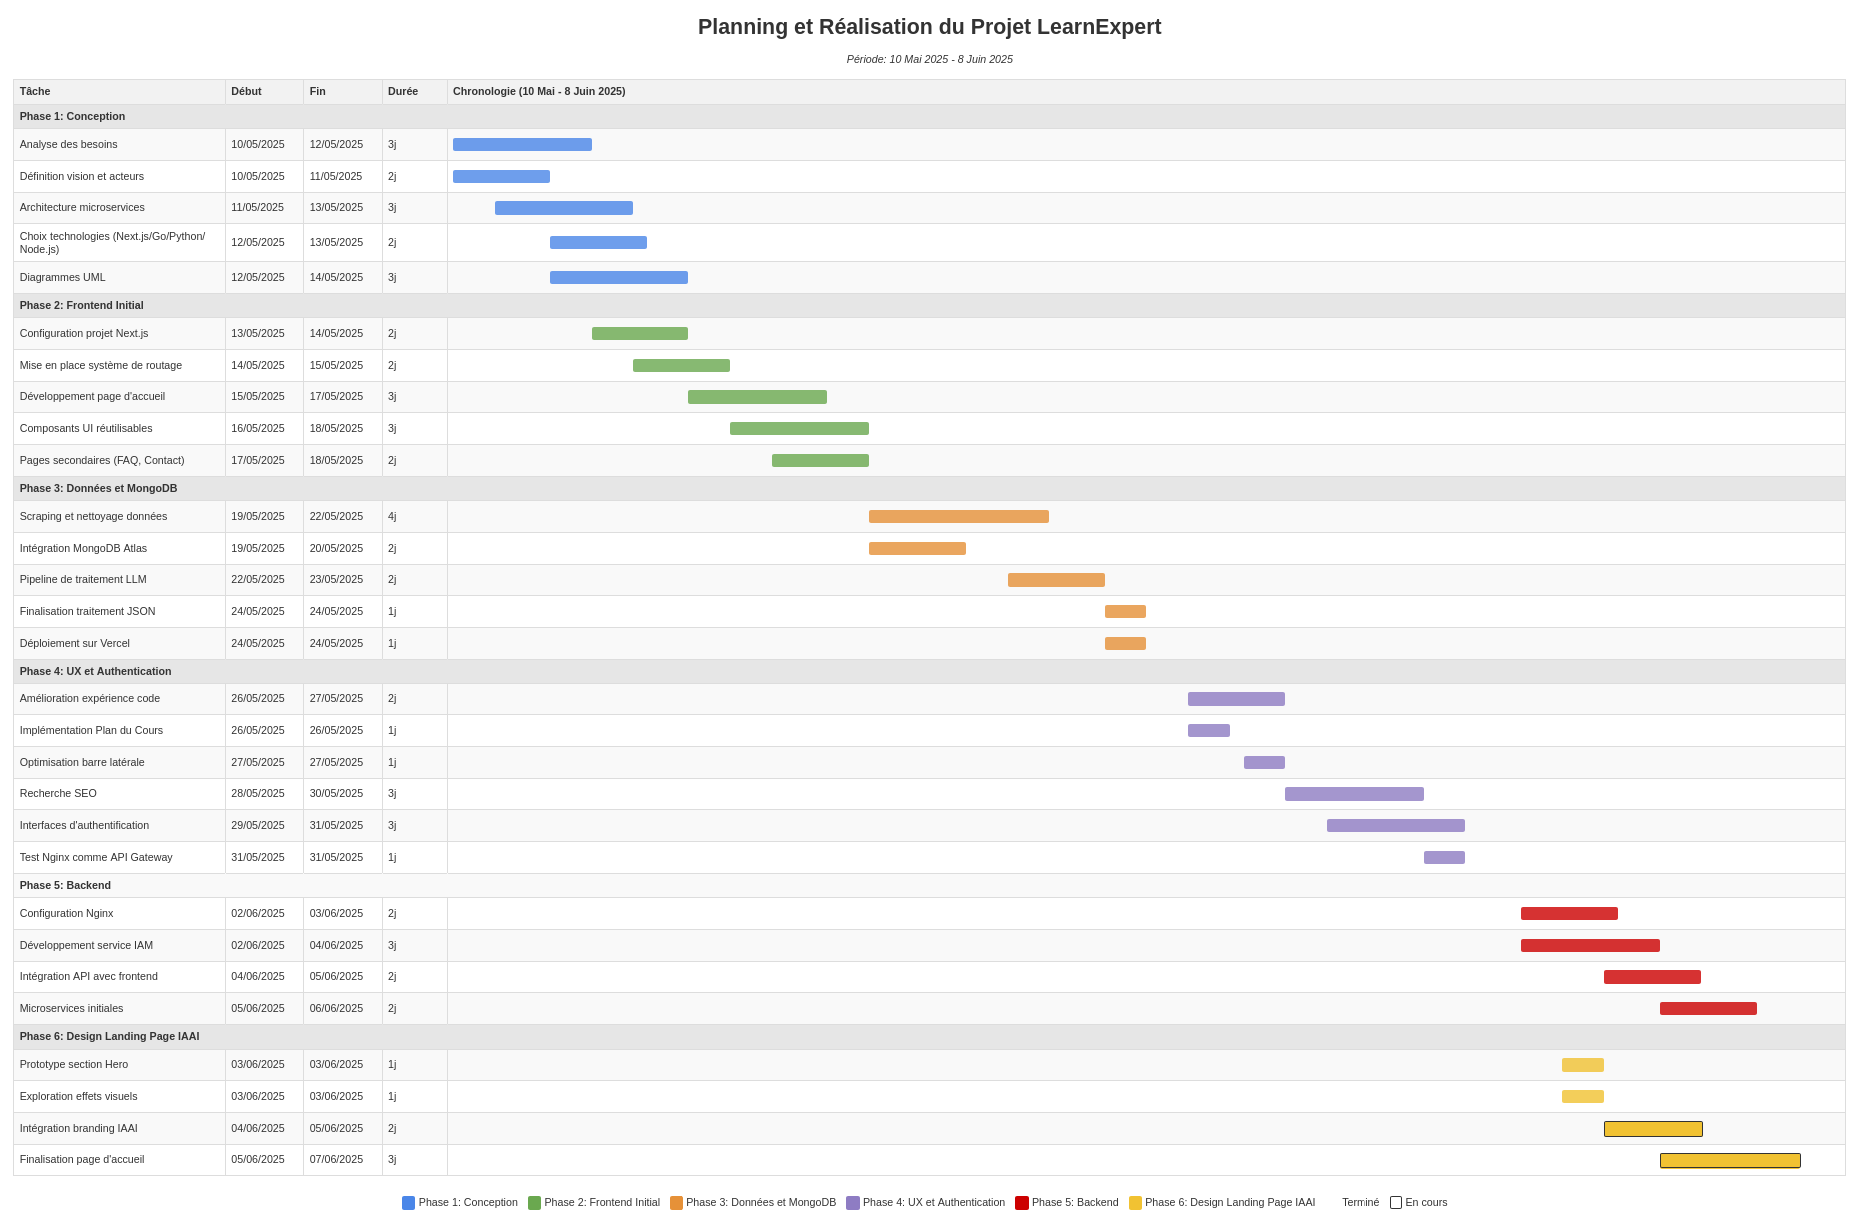
\includegraphics[width=0.9\textwidth,keepaspectratio]{images/gestion_projet/gantt_diagram.png}
  \caption{\textbf{Diagramme de Gantt} montrant la planification et la progression du projet.}
  \label{fig:gantt_diagram}
\end{figure}

Ce diagramme permet d'identifier clairement la durée totale du projet (du 10 mai au 8 juin 2025) ainsi que les périodes d'activité intense où plusieurs tâches se déroulent en parallèle. On peut notamment constater que les phases 1 à 3 (Conception, Frontend initial, Données et MongoDB) se déroulent principalement durant la première moitié du projet, tandis que les phases 4 à 6 (UX et Authentification, Backend, Design Landing Page) occupent la seconde moitié.

\subsection{Diagramme PERT}
Le diagramme PERT (Program Evaluation and Review Technique) complète le diagramme de Gantt en illustrant les dépendances entre les tâches et le chemin critique du projet.

\begin{figure}[htb]
  \centering
  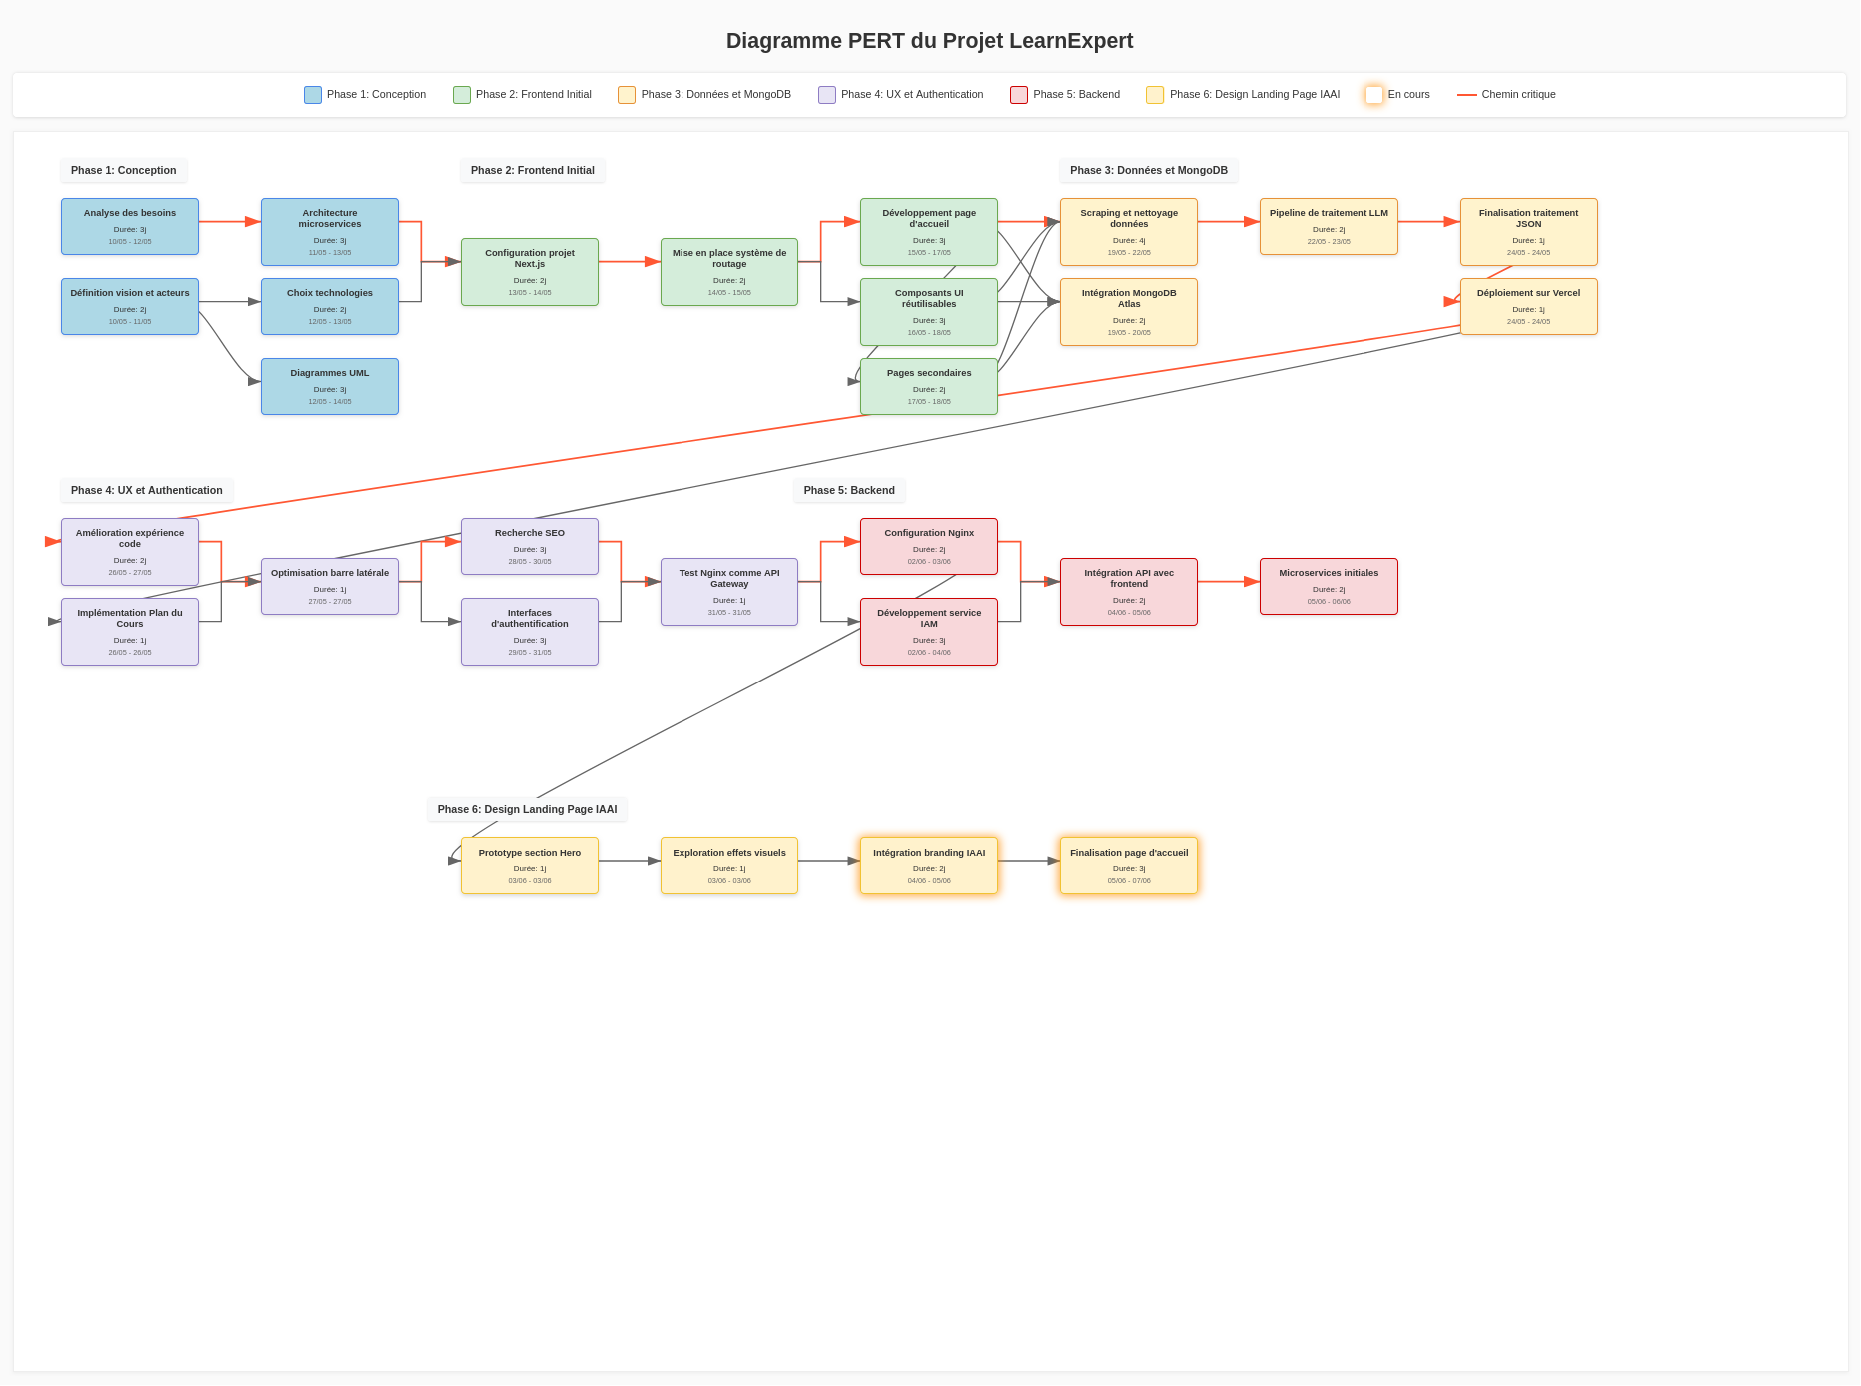
\includegraphics[width=0.9\textwidth,keepaspectratio]{images/gestion_projet/pert_diagram.png}
  \caption{\textbf{Diagramme PERT} montrant les relations et dépendances entre les tâches du projet.}
  \label{fig:pert_diagram}
\end{figure}

L'analyse du diagramme PERT permet de dégager plusieurs observations importantes :

\begin{itemize}[leftmargin=*,noitemsep,topsep=0pt]
  \item \textbf{Organisation modulaire} : Les tâches sont regroupées en six phases distinctes, chacune avec ses propres objectifs et livrables.
  
  \item \textbf{Dépendances inter-phases} : Certaines tâches de phases ultérieures dépendent de l'achèvement de tâches de phases antérieures, ce qui souligne l'importance de respecter les jalons intermédiaires.
  
  \item \textbf{Chemin critique} : Représenté en rouge, le chemin critique identifie les tâches dont tout retard impacterait directement la date de fin du projet. Il traverse notamment les phases de conception, de développement frontend, de pages secondaires, et s'étend jusqu'aux services backend.
  
  \item \textbf{Parallélisation des tâches} : Plusieurs activités peuvent être menées en parallèle, comme le développement des composants UI et la mise en place du système de routage, optimisant ainsi l'utilisation des ressources.
\end{itemize}

\subsection{Avantages de la Planification Visuelle}

L'utilisation combinée des diagrammes de Gantt et PERT présente plusieurs avantages significatifs pour la gestion du projet :

\begin{itemize}[leftmargin=*,noitemsep,topsep=0pt]
  \item \textbf{Communication claire} : Facilite la compréhension du planning par toutes les parties prenantes, techniques et non techniques.
  
  \item \textbf{Identification des risques} : Permet de repérer les zones de tension potentielles dans le planning, notamment les tâches sur le chemin critique.
  
  \item \textbf{Suivi de l'avancement} : Offre un référentiel visuel pour mesurer la progression réelle par rapport au planning initial.
  
  \item \textbf{Allocation des ressources} : Aide à l'optimisation de l'attribution des ressources humaines et techniques sur les différentes tâches.
  
  \item \textbf{Anticipation des dépendances} : Met en évidence les relations entre les tâches, permettant de préparer à l'avance les transitions entre phases.
\end{itemize}

La planification détaillée réalisée pour le projet LearnExpert constitue un élément essentiel pour assurer une exécution maîtrisée et respecter les délais fixés. Elle servira de référence tout au long du développement pour suivre l'avancement et ajuster les priorités si nécessaire.

\section{Conclusion}

Le cahier des charges présenté dans ce chapitre définit les fondements du projet LearnExpert, établissant clairement le contexte, les objectifs et les spécifications techniques nécessaires à sa réalisation. Face aux défis identifiés dans le secteur de l'éducation en ligne, la plateforme ambitionne d'apporter une solution innovante centrée sur l'apprentissage interactif de la programmation et des technologies web.

L'analyse approfondie des besoins fonctionnels et non fonctionnels a permis d'établir un cadre précis pour le développement, avec un accent particulier sur l'expérience utilisateur, la performance et la sécurité. La structure modulaire envisagée pour la plateforme favorisera son évolutivité et sa maintenance sur le long terme.

Le choix des technologies, notamment Next.js pour le frontend, une architecture microservices pour le backend, et l'utilisation de modèles de langage large pour le traitement des données, témoigne d'une approche moderne et adaptée aux exigences du projet. Cette sélection technique offre un équilibre optimal entre performance, flexibilité et facilité de développement, posant ainsi les bases solides pour la phase de conception et d'implémentation qui suivra.

Une planification rigoureuse du projet a été établie à l'aide des diagrammes de Gantt et PERT, permettant une visualisation claire des phases, des tâches et de leurs interdépendances. Cette organisation méthodique constitue un atout majeur pour le bon déroulement du projet dans les délais impartis.

Cette phase préparatoire constitue une étape cruciale dans le cycle de vie du projet, fournissant une vision claire et des directives précises pour guider efficacement les phases ultérieures de développement. 